\subsection{Checking}\label{subsec:checking}

% Outputting automata to UPPAAL, allows for checking of timed words, to determine whether they are accepted by the automaton generated from the regular expression. This can be done using UPPAAL's verifier, which simulates the transition system.

% The timed word itself is represented in the declarations section in UPPAAL. In order to check words containing values outside of the bounds of shorts, the type used by the timed word array containing types, uses a custom type that is defined to be of the same size as the integer representing clock values. Here we define two arrays. One containing the symbols, and one containing the times. The alphabet is represented by channels, as well as an automaton with transitions for each symbol, that also increase the index of the timed word arrays. During simulations, the clock ticks up until a symbol time is reached. When this happens, the automaton representing the alphabet takes the corresponding transition. This sends a signal though the channel of the same name, which allows a transition to be taken in the automaton representing the timed regular expression. A timed word is considered to be accepted by the timed regular expression, when the automaton representing the timed regular expression is able to reach a final state.

Using the UPPAAL output format, enables the user to make use of UPPAAL's model checking and verification capabilities.
By constructing a TA representing a given timed word, it is possible to verify that a given TRE satisfies the timing constraints of the timed word.
Given a timed word: $$(A, 0), (A, 2), (B, 3), (B, 3), (A, 8), (B, 12)$$
We can use the following TRE to look for the word ABBA in a span of 10 time units, which it should find starting at index 1: $$(ABBA)[0;10]$$
On such a small timed word, and a trivial TRE, it is easy to do manually, but with timed words with thousands or millions of timed characters, it is useful to have the ability to automate this with UPPAAL.

\subsubsection{Timed Automaton Representation}\label{subsubsec:ta_rep}
In UPPAAL, TAs are represented by a set of states and transitions connecting these states.
Both states and transitions have properties, but only the properties pertaining to transitions are relavant in this paper. Namely, Guards, Synchronizations and Updates, which are explained in UPPAAL's documentation \cite{UPPAAL}.
The TA shown on \cref{fig:ta_rep} is constructed from the TRE described above. For now, disregard the looping transition on the initial state and the endIndex variable on the last transition, as they will be explained in \cref{subsubsec:verifier}.

\vspace{0.75em}
\begin{center}
    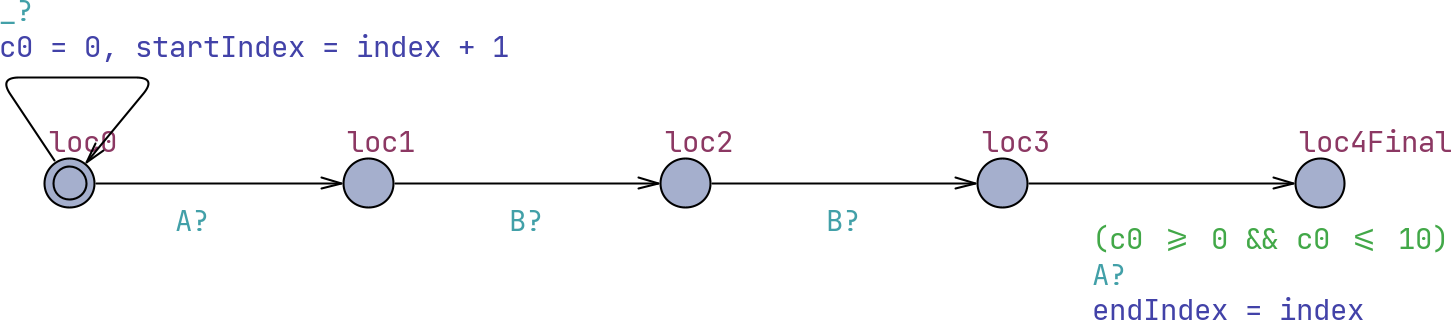
\includegraphics[width=\columnwidth]{Documents/Diagrams/CheckingFigures/checking_tarep.png}
    \captionof{figure}{TA constructed from the TRE $(ABBA)[0;10]$.}
    \label{fig:ta_rep}
\end{center}
\vspace{0.75em}

The word is recognized by the TA, if the execution terminates at a final state.
In the case of the TA on \cref{fig:ta_rep}, the only accepted word is ABBA, and it is only accepted if the 4 symbols appear within 10 time units of each other.

\vspace{.5\baselineskip plus 2pt}
The final state can only be reached by traversing the graph's transitions, and these transitions have been constructed to meet the requirements of the TRE. Each symbol in the TRE is converted into a datatype called a Channel \cite{UPPAAL}. While the documentation says they are used to synchronize processes (TA), the intuition in this paper, is that they are used to send and receive signals across channels. The syntax is as follows:

\vspace{0.5em}
\begin{itemize}
    \setlength\itemsep{0.2em}
    \item $x!$ - Outgoing signal (send)
    \item $x?$ - Incoming signal (receive)
\end{itemize}
\vspace{0.5em}

Where $x$ is any symbol. This syntax is used in Synchronizations on transitions. On \cref{fig:ta_rep}, each transition has an incoming synchronization label, meaning that each transition can only be traversed, when the corresponding signal is given. The outgoing signals will be administered by timed words. On the last transition in the TA, an additional Guard label is present, which represents the timing constraint. Along with an incoming signal, the clock $c0$ has to be within 10 time units for the transition to be taken.

\subsubsection{Timed Word Representation}\label{subsubsec:tw_rep}
In UPPAAL, timed words are represented by two arrays. One array for the symbols of the timed word, and another for the times. This way, the two arrays form pairs of symbols and their corresponding times. The timed word described above would be written like this:

\vspace{0.75em}
\begin{lstlisting}[basicstyle=\scriptsize]
    const string word[7] = {"A", "A", "B", "B", 
                            "A", "B", "\0"};
    clock_t times[7] = {0, 2, 3, 3, 8, 12, 13};
\end{lstlisting}
\captionof{lstlisting}{Timed word in UPPAAL.}
\label{lstlisting:timed_word}
\vspace{0.75em}

From this timed word, a TA can be constructed to interact with the other TA constructed from the TRE. This TA can be seen on \cref{fig:tw_rep}.

\vspace{0.75em}
\begin{center}
    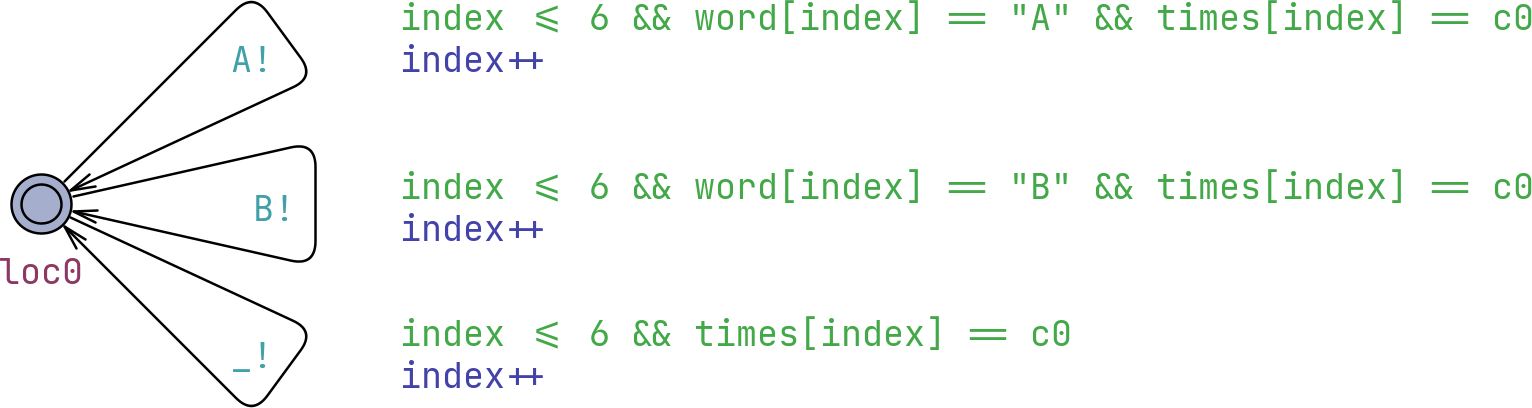
\includegraphics[width=\columnwidth]{Documents/Diagrams/CheckingFigures/checking_twrep.png}
    \captionof{figure}{Timed word TA for \cref{lstlisting:timed_word}. Positions heavily modified for visual clarity.}
    \label{fig:tw_rep}
\end{center}
\vspace{0.75em}

The TA consists of a single state, and one looping transition for each unique symbol in the timed word, plus an extra transition that matches any symbol.
Each transition has a Guard, a Synchronization and an Update. Take the transition for the symbol $A$.
It boils down to: ``\textit{If the current symbol is $A$ and the current time matches its timestamp (Guard), send a signal on channel $A$(Synchronization) and move to the next symbol (Update).}''
This is the case for all transitions, except the match-any transition, since it sends a signal for each symbol in the timed word. The signals sent by the outgoing Synchronizations are being received by the TA on \cref{fig:ta_rep}, which potentially progresses the TA. If there is a sequence of symbols in the timed word that matches the initial TRE, the TA should reach the final state. UPPAAL has a tool that makes this process of verification much simpler.

\subsubsection{Verifier}\label{subsubsec:verifier}
The verifier in UPPAAL can be used to check a multitude of properties of a given TA, but in this project, it is only used to check if the TA has reached a final state. \cref{lstlisting:query} shows the query for checking this for the TA on \cref{fig:ta_rep}.

\vspace{0.75em}
\begin{lstlisting}[basicstyle=\scriptsize]
    inf{ta0.startIndex >= 0 && (ta0.loc4Final)} : 
    ta0.startIndex, ta0.endIndex
\end{lstlisting}
\captionof{lstlisting}{Query for checking if a final state is reached.}
\label{lstlisting:query}
\vspace{0.75em}

All query syntax and semantics can be found on UPPAAL's documentation \cite{UPPAAL}, but this specific query is structured as follows:
\begin{lstlisting}[basicstyle=\scriptsize]
    operation{predicate} : subject
\end{lstlisting}
It finds the infimum of startIndex and endIndex shown in \cref{fig:ta_rep}, but only if startIndex is greater than or equal to 0 and the TA has reached a final state. The infimum operation finds the minimum value of the subject given the condition is true, which in this case finds the first occurence of $ABBA$ in the timed word.

\vspace{.5\baselineskip plus 2pt}
This is where the transitions, that were disregarded on \cref{fig:ta_rep} are used. The looping transition ensures the TA waits in the initial state until a possible match start is found in the timed word. The startIndex is set to the current index in the timed word plus one because the looping transition is only taken for non-matching symbols. Therefore, the last non-matching character will be right before the match.

\vspace{.5\baselineskip plus 2pt}
The endIndex is set to the current index of the timed word, when the TA reaches a final state. This means, the infimum operation finds the first and shortest match.

\vspace{.5\baselineskip plus 2pt}
The predicate for the infimum operation checks that the startIndex is greater than a certain value. To find the next match, this value can be set to the startIndex plus one of the previous match. This allows for a crude method of finding all matches on a timed word, one at a time.

\subsubsection{Shortcomings}\label{subsubsec:shortcomings}
We have encountered some limitations with UPPAAL, that we have had to work around.

% int sizes (shorts (summer))
% vi repræsenterer indices med floats, men uppaal er det int16
% clocks højeste værdi er 2^30-2, hvilket clasher med int16
% clock_t i typedef
% floating point clocks ??
\vspace{.5\baselineskip plus 2pt}
One of the most prominent issues we found is with UPPAAL's integer size, which is equal to an int16. This meant, that when implementing timed words, the elements in the times array had a maximum bound of 32.767, which is sufficient for smaller timed words, but they can contain millions of timed events. In UPPAAL, it is possible to define custom datatypes, and since we compare these times in the array to clocks, in the following example, we thought to define a datatype with the same size as the clock datatype.

\begin{lstlisting} [basicstyle=\scriptsize]
    word[index] == "A" && times[index] == c0
\end{lstlisting}

The UPPAAL documentation does not say much on the clock datatype, however, through trial and error we have found it to be of the size $2^{30}-2$ bits.
This further cements that the integer size is a bottleneck to our implementation, which limits us to a relatively small maximum bound for timed words.
With the actual size of clocks, we defined a new datatype called \verb|clock_t|, which has been used on \cref{lstlisting:timed_word}. It is defined to be the same size as the clock datatype, and declared as follows in the system declaration in UPPAAL:

\begin{lstlisting} [basicstyle=\scriptsize]
    typedef int[-1073741822,1073741822] clock_t;
\end{lstlisting}

This results in UPPAAL being able to handle much larger timed words.

% RAM issues (works fine on linux, nono on windows)
% output where match occurs
%   diagnostic trace gives
%   just output start and end indices